\documentclass[8pt]{beamer}
\usetheme{Dresden}
%\usecolortheme{beaver}
\usepackage[utf8]{inputenc}
\usepackage[spanish]{babel}
\usepackage{amsmath}
\usepackage{amsfonts}
\usepackage{amssymb}
\usepackage{graphicx}
\usepackage{booktabs}
%\usepackage{multirow}
%\usepackage{multicol}
\usepackage{subfig}
\usepackage{caption}
\usepackage{ragged2e}
\usepackage{parskip}
\usepackage{xcolor}
\usepackage{tcolorbox}
\usepackage{braket}
\usepackage{tikz}
\usepackage{colortbl}
\captionsetup{font=scriptsize,labelfont=scriptsize}
\tcbset{colbacktitle=blue!75!black, colframe=blue!25!black, colback=blue!20!white, fonttitle=\bfseries}
\author[]
{Sistema de Detección y Evasión de Colisiones basado en Visión Computacional para Vehículos Autónomos\\
\vspace{2em}
Rubén Martínez González}
\title[Protocolo de tesis]{Protocolo de tesis}
%\setbeamercovered{transparent} 
\setbeamertemplate{navigation symbols}{}
\setbeamertemplate{page number in head/foot}[totalframenumber]
\institute[FMAT, UADY]{Facultad de Matemáticas, UADY}
\date{}
\titlegraphic{
    \vspace{1em}
    \hfill
    
\includegraphics[width=1.5cm]{img/uady.png}
    \hspace{1em}
    
\includegraphics[width=1.5cm]{img/fmat.png}
}
\subject{Seminario de investigación}
\begin{document}

    \begin{frame}
        \titlepage
    \end{frame}

%    \begin{frame}{Contenido}
%        \tableofcontents
%    \end{frame}


    \section{Introducción}
    \begin{frame}{Introducción}
        \begin{itemize}
            \item La tecnología de vehículos autónomos representa un logro significativo en la revolución del transporte.
            \item Desarrollar sistemas ‘inteligentes’ que permitan a estos vehículos aprender a conducir de manera autónoma
            \item Detectar posibles colisiones y reaccionar de manera similar a un humano
            \item Sistema de detección y evasión de colisiones basado en visión computacional
            \item La detección y respuesta a situaciones de peligro, como colisiones inminentes, siguen siendo un desafío complejo.
        \end{itemize}
    \end{frame}


    \section{Problemática}
    \begin{frame}{Contexto y problemática}
        \begin{itemize}
            \item El desafío primordial reside en dotar a estos vehículos con la capacidad de identificar y reaccionar ante situaciones de riesgo de manera precisa
            \item La detección temprana de posibles colisiones, amenazas viales es un aspecto esencial para garantizar la seguridad
            \item La visión computacional, utilizando las cámaras de video y sensores, se presenta como una estrategia central para esta detección
            \item Existen desafíos tecnológicos significativos en la identificación y procesamiento oportuno de dichos eventos
        \end{itemize}
    \end{frame}
    \begin{frame}{Preguntas de investigación}
        \begin{itemize}
            \item ¿Cómo se puede implementar un sistema de detección y evasión de colisiones basado en visión computacional para vehículos autónomos?
            \item ¿Cómo se puede mejorar la precisión y la velocidad de detección de posibles colisiones mediante técnicas avanzadas de visión computacional?
            \item ¿Cuál es el impacto de la integración de múltiples sensores en la detección y evasión de colisiones para vehículos autónomos?
        \end{itemize}
    \end{frame}
    \begin{frame}{Hipótesis}
        \("\)El desarrollo de un sistema de detección y evasión de colisiones basado en visión computacional en vehículos autónomos
        proporcionará a estos la capacidad de anticipación y respuesta ante posibles situaciones de riesgo\("\)
    \end{frame}


    \section{Objetivos}
    \begin{frame}{Objetivo general}
        Desarrollar un sistema de detección y evasión de colisiones basado en visión computacional para vehículos autónomos en simulación,
    \end{frame}
    \begin{frame}{Objetivos específicos}
        \begin{itemize}
            \item Modelar un ambiente de simulación donde un vehiculo circule por calles transitadas.
            \item Obtener datos de los sensores del vehiculo en simulación.
            \item Interpretar los datos de los sensores mediante técnicas de visión computacional.
            \item Procesar los datos y aprender a reaccionar.
        \end{itemize}
    \end{frame}


    \section{Estado del arte}
    \begin{frame}{Trabajos previos relacionados}
        Bachute, M. R., and Subhedar, J. M. Autonomous driving architectures: insights of
        machine learning and deep learning algorithms. Machine Learning with Applications 6
        (2021), 100164.\\
        \begin{figure}[!ht]
            \begin{subfigure}
                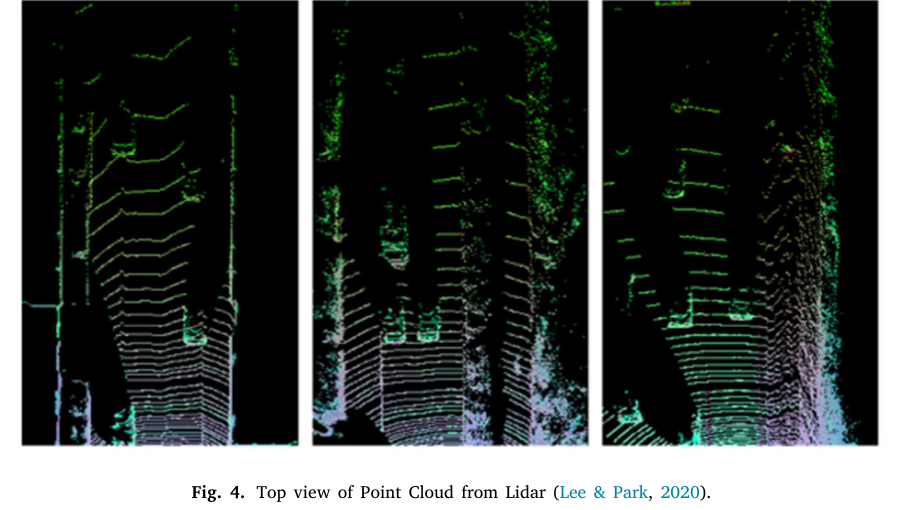
\includegraphics[width=0.3\textwidth]{img/12Screenshot_20231106_142954}\label{fig:12}
            \end{subfigure}
            \begin{subfigure}
                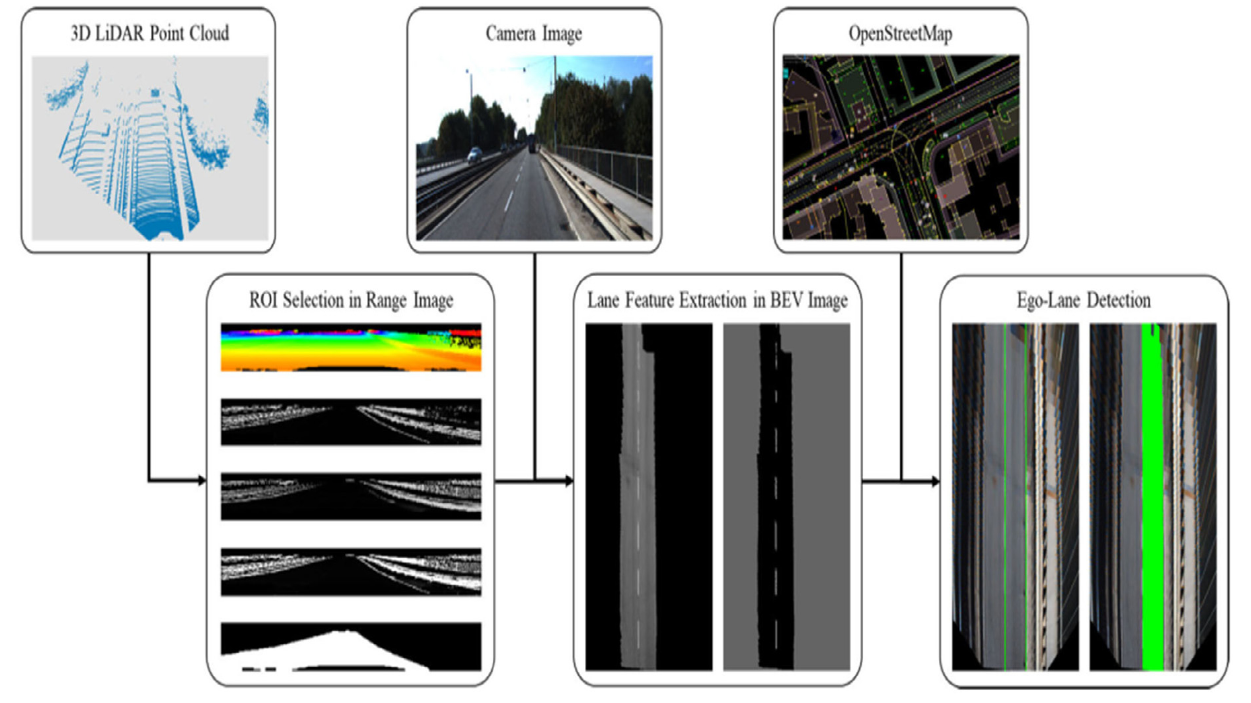
\includegraphics[width=0.3\textwidth]{img/14 Screenshot_20231106_143419}\label{fig:14}
            \end{subfigure}
            \begin{subfigure}
                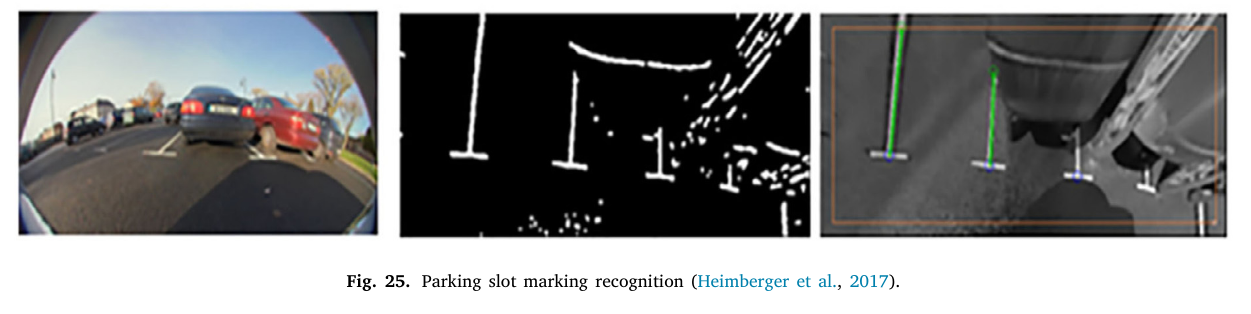
\includegraphics[width=0.3\textwidth]{img/16Screenshot_20231106_143701}\label{fig:16}
            \end{subfigure}
        \end{figure}
        Ofrece una visión general de cómo se aplican algoritmos de Aprendizaje Automático y Aprendizaje
        Profundo en sistemas de conducción autónoma
    \end{frame}

    \begin{frame}{Trabajos previos relacionados}
        Cai, P., Wang, H., Huang, H., Liu, Y., and Liu, M. Vision-based autonomous car racing
        using deep imitative reinforcement learning. IEEE Robotics and Automation Letters 6, 4
        (2021), 7262–7269.\\
        \begin{figure}[!ht]
            \begin{subfigure}
                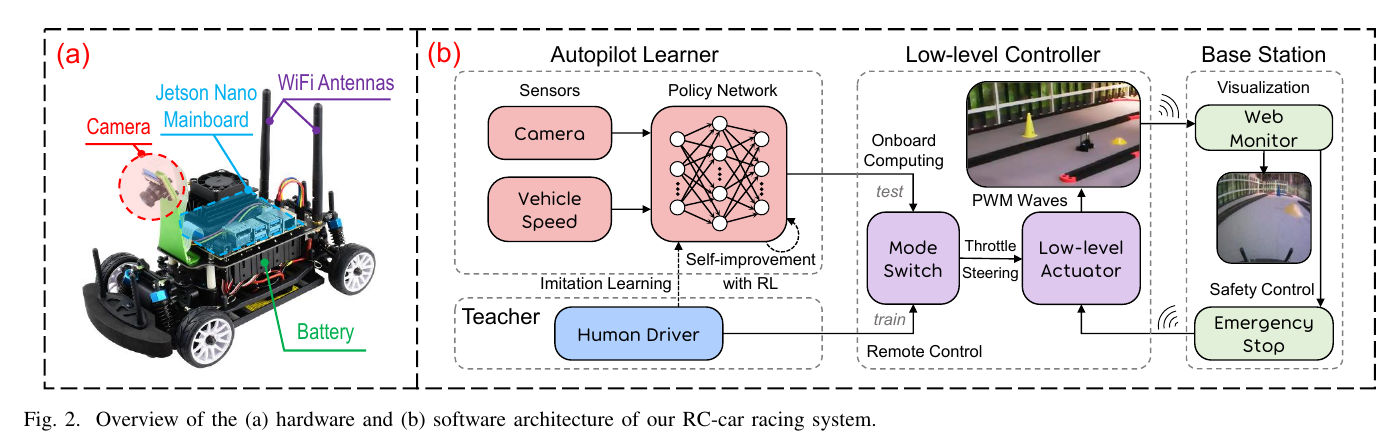
\includegraphics[width=0.8\textwidth]{img/21}\label{fig:21}
            \end{subfigure}
        \end{figure}
        se presenta un enfoque general de aprendizaje profundo imitativo y de refuerzo (DIRL) que logra el automovilismo
        autónomo ágil utilizando entradas visuales.
    \end{frame}

    \begin{frame}{Trabajos previos relacionados}
        Althoff, M., Stursberg, O., and Buss, M. Model-based probabilistic collision detection in
        autonomous driving. IEEE Transactions on Intelligent Transportation Systems 10, 2 (2009),
        299–310.\\
        \begin{figure}[!ht]
            \begin{subfigure}
                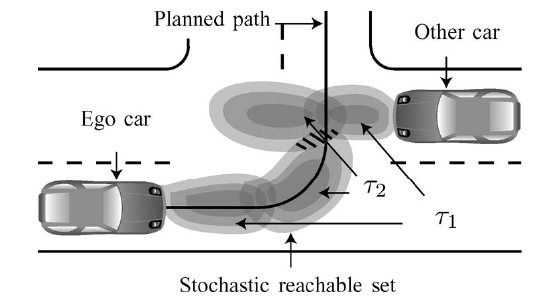
\includegraphics[width=0.3\textwidth]{img/31}\label{fig:31}
            \end{subfigure}
            \begin{subfigure}
                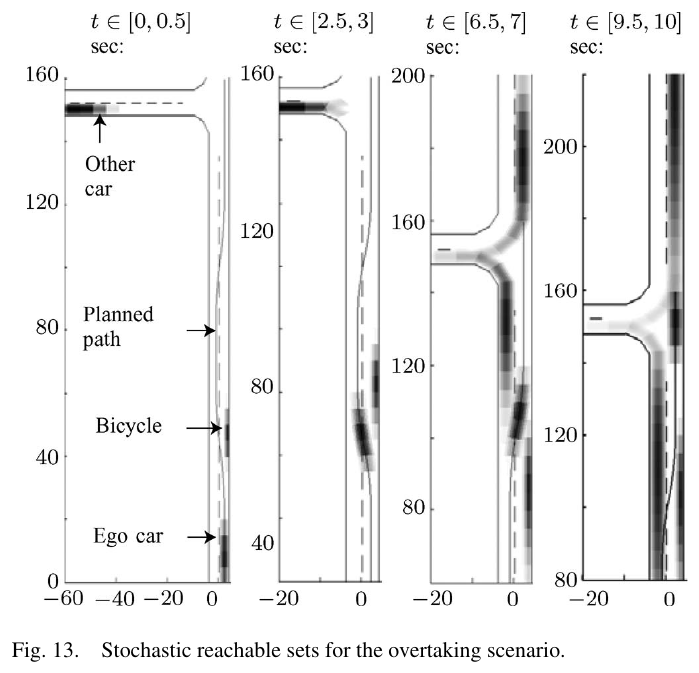
\includegraphics[width=0.3\textwidth]{img/33}\label{fig:33}
            \end{subfigure}
            \begin{subfigure}
                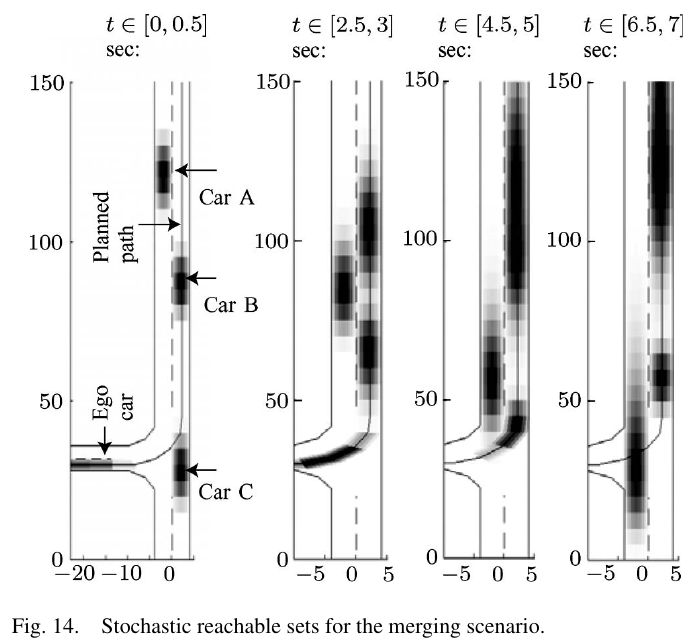
\includegraphics[width=0.3\textwidth]{img/34}\label{fig:34}
            \end{subfigure}
        \end{figure}
        Se centra en la seguridad de los caminos planificados para autos autónomos en relación con otros participantes en el tráfico.
        Se predice la ocupación de la carretera por otros vehículos de manera estocástica.
    \end{frame}

    \begin{frame}{Trabajos previos relacionados}
        APavel, M. I., Tan, S. Y., and Abdullah, A. Vision-based autonomous vehicle systems
        based on deep learning: A systematic literature review. Applied Sciences 12, 14 (2022),
        6831.\\
        \begin{figure}[!ht]
            \begin{subfigure}
                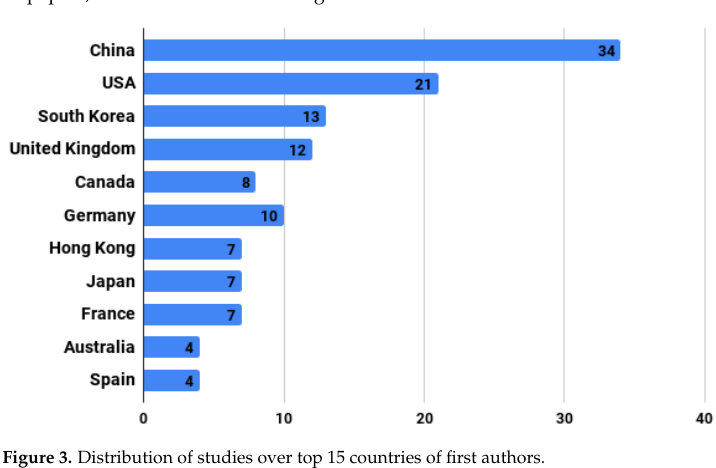
\includegraphics[width=0.4\textwidth]{img/74}\label{fig:74}
            \end{subfigure}
            \begin{subfigure}
                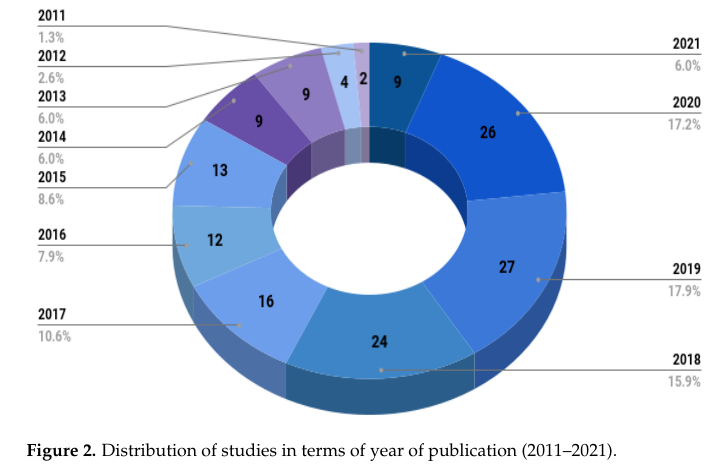
\includegraphics[width=0.4\textwidth]{img/73}\label{fig:73}
            \end{subfigure}
        \end{figure}
        El artículo realiza una revisión sistemática de la literatura sobre el uso del aprendizaje profundo en AVS durante la última década.

    \end{frame}
    \begin{frame}{Trabajos previos relacionados}
        Alam, A., Jaffery, Z. A., and Sharma, H. A cost-effective computer vision-based vehicle
        detection system. Concurrent Engineering 30, 2 (2022), 148–158.\\
        \begin{figure}[!ht]
            \begin{subfigure}
                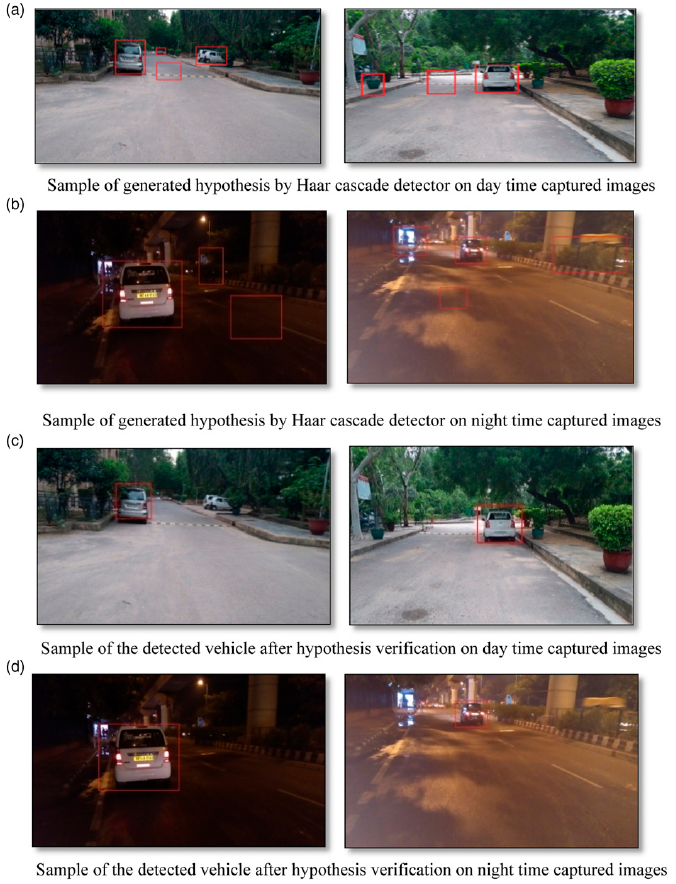
\includegraphics[width=0.3\textwidth]{img/84}\label{fig:84}
            \end{subfigure}
            \begin{subfigure}
                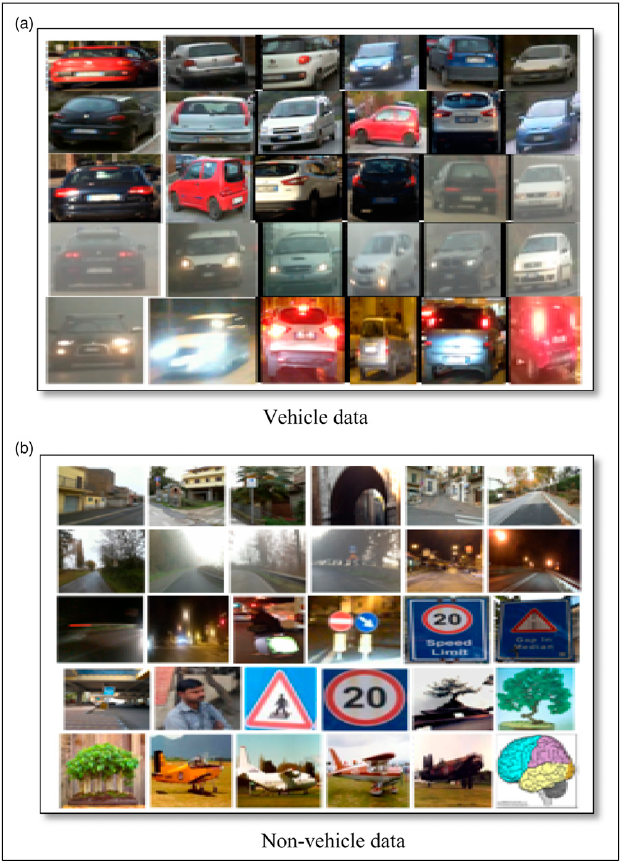
\includegraphics[width=0.3\textwidth]{img/82}\label{fig:86}
            \end{subfigure}
        \end{figure}
        Propone un sistema de detección de vehículos basado en visión por computadora que utiliza un algoritmo
        de Gentle Adaptive Boosting con características tipo Haar para generar hipótesis de vehículos de manera rápida.
    \end{frame}

    \begin{frame}{Tabla comparativa}
        \begin{table}
            \footnotesize
            \begin{tabular}{|p{3cm}|p{1.2cm}|p{1.2cm}|p{1.2cm}|p{1.2cm}|p{1.2cm}|}
                \hline
                \textbf{Características}
                & \textbf{Autonomous Driving Architectures}
                & \textbf{Vision-based Autonomous Car Racing}
                & \textbf{Model-based Probabilistic Collision Detection}
                & \textbf{Vision-based Autonomous Vehicle Systems}
                & \textbf{Cost-effective Vehicle Detection System} \\
                \hline
                Uso de algoritmos de Aprendizaje Automático y Aprendizaje Profundo & X &   &   & X &   \\
                \hline
                Enfoque en la conducción autónoma                                  & X & X & X & X & X \\
                \hline
                Ventajas de la conducción autónoma                                 & X &   &   &   &   \\
                \hline
                Complejidad de los sistemas de conducción autónoma                 & X &   &   &   &   \\
                \hline
                Análisis de tareas en la conducción autónoma                       & X &   &   &   &   \\
                \hline
                Evaluación y comparación de algoritmos                             & X & X &   &   &   \\
                \hline
                Predicción estocástica de ocupación de la carretera                &   &   & X &   &   \\
                \hline
                Eficiencia en cálculos intensivos                                  &   & X & X &   &   \\
                \hline
                Utilización de cámaras RGB como sensores principales               &   & X &   & X &   \\
                \hline
                Detección de vehículos en conducción autónoma                      &   &   &   &   & X \\
                \hline
            \end{tabular}
        \end{table}
    \end{frame}


    \section{Metodología}
    \begin{frame}{Metodología}
        La metodología propuesta se fundamenta en un enfoque iterativo que abarca diversas etapas para la implementación del sistema de detección
        y evasión de colisiones en vehículos autónomos.
        \begin{itemize}

            \item Se establecerá un entorno de simulación realista que refleje las condiciones de tráfico habituales.
            \item Adquisición y procesamiento de datos provenientes de los sensores de dicho entorno simulado.
            \item Diseño y la implementación de algoritmos de visión computacional para la detección temprana de eventos críticos en tiempo real.
            \item Estos algoritmos serán sometidos a un proceso de entrenamiento y ajuste utilizando técnicas de aprendizaje automático.
            \item Se llevarán a cabo pruebas para validar la efectividad y la precisión del sistema propuesto en situaciones simuladas de riesgo vial.
        \end{itemize}
    \end{frame}


    \section{Calendario}
    \begin{frame}{Calendario de actividades}
        \begin{center}
            \resizebox{\textwidth}{!}{
                \begin{tabular}{|p{3cm}|p{1cm}|p{1cm}|p{1cm}|p{1cm}|p{1cm}|p{1cm}|p{1cm}|}
                    \hline
                    \textbf{Actividad} & \multicolumn{7}{c|}{\textbf{Duración}} \\
                    \hline
                    & \multicolumn{1}{p{1cm}|}{Dic}
                    & \multicolumn{1}{p{1cm}|}{Ene}
                    & \multicolumn{1}{p{1cm}|}{Feb}
                    & \multicolumn{1}{p{1cm}|}{Marz}
                    & \multicolumn{1}{p{1cm}|}{Abr}
                    & \multicolumn{1}{p{1cm}|}{May}
                    & \multicolumn{1}{p{1cm}|}{Jun}
                    \\
                    \hline
                    Investigación Preliminar                    & \cellcolor{gray!30} & \cellcolor{gray!30} &                     &                     &                     &                     &                     \\
                    \hline
                    Diseño y Configuración del Entorno Simulado &                     & \cellcolor{gray!30} & \cellcolor{gray!30} & & & & \\
                    \hline
                    Adquisición y Procesamiento de Datos        &                     &                     &                     & \cellcolor{gray!30} & \cellcolor{gray!30} & \cellcolor{gray!30} & \\
                    \hline
                    Desarrollo y Entrenamiento de Algoritmos    &                     &                     &                     &                     & \cellcolor{gray!30} & \cellcolor{gray!30} & \cellcolor{gray!30} \\
                    \hline
                    Evaluación y Ajuste del Sistema             &                     &                     &                     &                     &                     & \cellcolor{gray!30} & \cellcolor{gray!30} \\
                    \hline
                    Documentación y Análisis de Resultados      &                     &                     &                     &                     &                     &                     & \cellcolor{gray!30} \\
                    \hline
                    Redacción y Presentación de la Tesis        &                     &                     &                     &                     &                     &                     & \cellcolor{gray!30} \\
                    \hline
                \end{tabular}
            }
        \end{center}
    \end{frame}


    \section{Referencias}
    \begin{frame}{Referencias bibliográficas}
        \\[1] Alam, A., Jaffery, Z. A., and Sharma, H. A cost-effective computer vision-based vehicle
        detection system. Concurrent Engineering 30, 2 (2022), 148–158.
        \\[2] Althoff, M., Stursberg, O., and Buss, M. Model-based probabilistic collision detection in
        autonomous driving. IEEE Transactions on Intelligent Transportation Systems 10, 2 (2009),
        299–310.
        \\[3] Bachute, M. R., and Subhedar, J. M. Autonomous driving architectures: insights of
        machine learning and deep learning algorithms. Machine Learning with Applications 6
        (2021), 100164.
        \\[4] Cai, P., Wang, H., Huang, H., Liu, Y., and Liu, M. Vision-based autonomous car racing
        using deep imitative reinforcement learning. IEEE Robotics and Automation Letters 6, 4
        (2021), 7262–7269.
        \\[5] Pavel, M. I., Tan, S. Y., and Abdullah, A. Vision-based autonomous vehicle systems
        based on deep learning: A systematic literature review. Applied Sciences 12, 14 (2022),
        6831.

    \end{frame}
    
    \begin{frame}
        \titlepage
    \end{frame}
    
\end{document}
%no te da pena? ño